\documentclass{article}
\usepackage[utf8]{inputenc}
\usepackage[hidelinks]{hyperref}
\usepackage[spanish]{babel}
\usepackage[left=2cm,right=2cm,top=2cm,bottom=2cm]{geometry}
\usepackage{graphicx}
\usepackage{pdflscape}
\usepackage{listings}

\lstset {
    frame = single,
    breaklines = true
}

\begin{document}
\begin{titlepage}
\title{\textbf{
    {\Huge Práctica 2: Procesos ETL en un Data Mart}\\
    {\Large Almacenes y Minería de Datos}
}}
\author{
    Pedro Allué Tamargo (758267)
    \and
    Cristina Oriol García (755922)
    \and
    Alejandro Paricio García (761783)
}
\date{\today}
\clearpage\maketitle
\thispagestyle{empty}
\end{titlepage}

% Index
\tableofcontents


\newpage
\section{Introducción}

Tras el desarrollo del \textit{Data Mart} de vuelos comerciales en la práctica anterior se ha procedido al siguiente paso: la población del almacén de datos con datos reales. En esta práctica se va a explorar el concepto de proceso \textit{ETL}. Se va a diseñar e implementar el proceso \textit{ETL} para insertar los datos en el almacén.


\section{Modificación del esquema en estrella existente}

Se ha modificado el esquema en estrella de la práctica anterior para añadir información acerca de las ciudades en las que se encuentra el aeropuerto. Las modificaciones se centran en la dimensión \textit{Aeropuerto}. Se han añadido dos atributos que indican el número de habitantes de la ciudad y la zona horaria de la misma: \texttt{ciudadNumHabitantes} y \texttt{ciudadTimeZone}, respectivamente. También en esta dimensión se ha eliminado el atributo \texttt{codigoAeropuerto} ya que con los conjuntos de datos utilizados no se podía obtener. Al querer incluir la idea de código del aeropuerto que se pretendía obtener en la práctica anterior, se terminó dejando como identificador numérico del aeropuerto el código del mismo.\\
Durante la labor de búsqueda de los datos se encontraron problemas relacionados con los aviones. En esta dimensión se había decidido considerarlos como los aviones que realizan los vuelos, manteniendo su código de cola y modelo. Con los conjuntos de datos utilizados no había forma de obtener esa información y por lo tanto se ha mantenido en el esquema pero en su posterior traducción a \textit{SQL} se permitirán valores nulos ya que en un futuro es probable que se encuentren estos valores y se puedan asociar a la dimensión avión.\\
En la tabla de hechos (vuelos) se ha eliminado el hecho \texttt{tiempoTotalVuelo} ya que era redundante con el atributo \texttt{tiempoRealVuelo}, y no tenía el interés necesario para almacenarlo.\\
En la dimensión hora se ha eliminado el atributo \texttt{timeZone} ya que en esta práctica se pedía que se añadiera esa información a la dimensión de aeropuertos.\\
En la dimensión fecha se ha realizado una eliminación de atributos que dependían del calendario festivo.\\
Por lo tanto, el esquema en estrella modificado se puede observar en la Figura \ref{fig:esquema_estrella_modificado}.\\

De cara a la implementación \textit{SQL} se ha modificado el código de la práctica anterior para reflejar los cambios comentados anteriormente (Código \ref{list:codigoSQL}).\\

\newpage
\section{Proceso ETL}

\subsection{Planteamiento y diseño}
Se pide la implementación de un proceso ETL que realice una única carga de datos al almacén de datos derivado de las modificaciones realizadas al esquema en estrella de la práctica anterior. Debido al tipo de carga, no va existir una carga incremental, lo que variará el enfoque tomado para desarrollar el proceso ETL, pero se comentará a lo largo del informe alguna opción a considerar en caso de tratarse de esta última. Además, debido al conocimiento previo de uno de los miembros de KNIME, se tomaría como herramienta para el desarrollo, ya que eso facilitaría el lograr un resultado apropiado.\\

El primer tema tratado es la obtención y extracción de datos de las fuentes de información. Siguiendo las consideraciones dadas por el enunciado, se consultaron las fuentes \textbf{GeoNames}\footnote{http://www.geonames.org/,http://download.geonames.org/export/dump/}, una base de datos geográfica, y \textbf{RITA}\footnote{http://www.transtats.bts.gov} (Research and Innovative Technology Administration), que proporciona información de vuelos comerciales en Estados Unidos. Se observó que la información contenida en ambas era suficiente como para obtener los datos de los vuelos, las aerolíneas, aeropuertos de origen y destino, así como sus ciudades y estados con su población y zona horaria, completándose los requisitos del enunciado de la práctica 2. Una información faltante respecto a la incluida en el esquema en estrella de la práctica anterior eran los modelos de los aviones, tuvo que extraerse del esquema. No suponía un gran problema dado a que no se incluía como uno de los requisitos del almacén, sino que se añadió debido a que podía ser interesante para el análisis. No obstante, de haberse contado con esa información, podría incluirse en el mismo. Decididas las fuentes de información, se obtendrían los datos descargando la información directamente de las bases de datos anteriores en formato csv.\\

El siguiente paso sería la limpieza y conformado de los datos. Además, se planificaría a grandes rasgos cómo se iban a generar los módulos que obtenían la información en los formatos deseados. También se llevó a cabo la división del trabajo y se decidió quién se encargaría de qué parte, partiendo entre obtención de los datos de aeropuertos y su ciudad y el resto de información de los vuelos, contenida únicamente en la fuente RITA. Más adelante se detectarían casos especiales en los datos, debido principalmente a la no coincidencia de los datos de ambas fuentes en casos específicos, lo que se resolvió durante la implementación. Por ejemplo, aeropuertos con un código de estado distinto a la ciudad en la que se encuentran, lo que se daba, por ejemplo, en algunas localizaciones pertenecientes a Estados Unidos pero fuera del territorio continental.\\

Finalmente se procedería con la implementación y el poblado del almacén de datos, seguida de la redacción del informe. De la implementación en adelante se detalla en mayor medida, incluidos los problemas encontrados, en los siguientes apartados.\\

Si se quisiera realizar la carga de los datos de manera incremental se debería automatizar la ejecución del proceso \textit{ETL}. Para ello los ficheros de datos se deberían marcar con un \textit{timestamp} para conocer la fecha de la última ejecución del proceso. El \textit{script} que ejecute la carga incremental cogerá los datos a partir de esa fecha y se los pasará al proceso \textit{ETL}. Esta automatización podría conseguirse utilizando alguna herramienta como \textit{cron} en sistemas \textit{UNIX}.\\
 
\newpage
\subsubsection{Conjuntos de datos}

Los conjuntos de datos utilizados se corresponden con los propuestos en el enunciado de la práctica.\\
Para obtener la información acerca de las ciudades se ha utilizado el conjunto de datos \textit{US} de \textit{GeoNames\footnote{\url{http://download.geonames.org/export/dump/}}}.\\
Para obtener la información acerca de los vuelos, se ha obtenido un volcado de la base de datos de \textit{RITA} utilizando el enlace: \url{https://www.transtats.bts.gov/DL_SelectFields.asp?Table_ID=237}. Este enlace ofrece al usuario la posibilidad de elegir qué columnas aparecerán en el fichero de salida.\\

\subsubsection{Tratamiento de los vuelos}
De la base de datos \textit{RITA} comentada anteriormente se han obtenido los datos que conformaran las tablas \textit{Vuelos, Aeropuertos, Aerolíneas}.\\
En el fichero de \textit{76480265\_T\_ONTIME\_MARKETING.csv}(vuelos) las columnas son:
    \begin{itemize}
        \item ORIGIN\_AIRPORT\_ID: id aeropuerto origen.
        \item DEST\_AIRPORT\_ID: id aeropuerto destino.
        \item MKT\_UNIQUE\_CARRIER: id aerolínea.
        \item OP\_UNIQUE\_CARRIER: id operador.
        \item YEAR: año del vuelo.
        \item QUARTER: cuatrimestre del año del vuelo.
        \item MONTH: mes del vuelo.
        \item DAY\_OF\_MONTH: día del mes del vuelo.
        \item DAY\_OF\_WEEK: día de la semana del vuelo.
        \item FL\_DATE: fecha del vuelo en formato año-mes-día.
        \item TAIL\_NUM: identificador del avión con el que se realiza el vuelo.
        \item ORIGIN\_CITY\_NAME: nombre de la ciudad de origen.
        \item DEST\_CITY\_NAME: nombre de la ciudad de destino.
        \item ORIGIN\_STATE\_NM: nombre del estado de origen.
        \item DEST\_STATE\_NM: nombre del estado de destino.
        \item CRS\_DEP\_TIME: tiempo planeado de salida.
        \item CRS\_ARR\_TIME: tiempo planeado de llegada.
        \item DEP\_TIME: tiempo real de salida.
        \item ARR\_TIME: tiempo real de llegada.
        \item DEP\_DELAY\_NEW: diferencia en minutos entre la hora de salida real y la planeada, en caso de adelanto de los vuelos es un número negativo.
        \item ARR\_DELAY\_NEW: diferencia en minutos entre la hora de llegada real y la planeada, en caso de adelanto de los vuelos es un número negativo.
        \item CRS\_ELPSED\_TIME: tiempo de vuelo en minutos planeado.
        \item ACTUAL\_ELAPSED\_TIME: tiempo real de vuelo en minutos.
        \item AIR\_TIME: tiempo en minutos que el avión está volando.
    \end{itemize}
    
Para la tabla aeropuerto se ha utilizado el campo \textit{OriginAirportID} que contiene el identificador único asignado a cada aeropuerto y que vincula al fichero \textit{L\_AIRPORT\_ID} que contiene el campo \textit{Description} (nombre de cada aeropuerto). En el fichero de vuelos se encuentran dos referencias a este fichero \textit{ORIGIN\_AIRPORT\_ID, DEST\_AIRPORT\_ID} que referencian el aeropuerto de origen y el de destino.\\
Para las tablas Aerolínea y Operadora se tienen los campos \textit{ MKT\_UNIQUE\_CARRIER,  OP\_UNIQUE\_CARRIER} respectivamente que contienen el identificador único asignado a cada aerolínea u operadora. Estas columnas nos relacionan el fichero de vuelos con el fichero \textit{L\_UNIQUE\_CARRIERS} que también contiene el campo \textit{Description} en el que se encuentra el nombre de la aerolínea. En el fichero de vuelos se encuentran dos referencias a este fichero \textit{MKT\_UNIQUE\_CARRIER, OP\_UNIQUE\_CARRIER} que referencian a la aerolínea y a la operadora del vuelo.\\


\newpage
\subsubsection{Tratamiento de las ciudades y los aeropuertos}
\label{4.1.2}
Para la obtención relacionada con los aeropuertos y su localización, es decir, su estado, ciudad y la población de la misma entre otros, se han utilizado los siguientes ficheros:

\begin{itemize}
    \item \textit{L\_AIRPORT\_ID.csv}: Contiene la información del identificador numérico de cada vuelo, su nombre y su estado, descrito previamente.
    \item \textit{76480265\_T\_ONTIME\_MARKETING.csv}: Contiene, entre otros atributos descritos anteriormente, el código, nombre de la ciudad y nombre del estado de los aeropuertos de origen y destino de cada vuelo.
    \item \textit{cities500.txt}: Obtenido de la fuente de datos de \textit{GeoNames} \url{http://download.geonames.org/export/dump/}, concretamente del fichero cities500.zip. El mismo contiene información acerca de todas las ciudades almacenadas en \textit{GeoNames} con 500 o más habitantes. El conjunto de atributos del mismo se compone de:
        \begin{itemize}
            \item geonameid: Id entero de la base de datos de \textit{GeoNames}.
            \item name: Nombre del punto geográfico (\textit{utf8}) \texttt{varchar(200)}.
            \item asciiname: Nombre del punto geográfico en caracteres \textit{ascii}, \texttt{varchar(200)}.
            \item alternatenames: Nombres alternativos separados por coma, obtenidos automáticamente por medio de transliteración ~\cite{Transliteracion}.
            \item latitude: Latitud del punto geográfico en grados decimales.
            \item longitud: Longitud del punto geográfico en grados decimales.
            \item feature class: Identificador de \textit{GeoNames} de la clase del punto geográfico, ver \url{http://www.geonames.org/export/codes.html}.
            \item feature code: Código de \textit{GeoNames} del del tipo de elemento dentro de una clase del punto geográfico, ver \url{http://www.geonames.org/export/codes.html}.
            \item country code: Código del país, definido por el estándar \textit{ISO-3166}~\cite{ISO3166} (2 letras). 
            \item cc2: Códigos del país alternativos, definidos por el estándar anterior.
            \item admin1: Para los puntos estadounidenses, se corresponde con el código \textit{FIPS}~\cite{FIPS}.
            \item admin2: Código para la segunda división administrativa, un condado en Estados Unidos.
            \item admin3: Código para el tercer nivel de división administrativa.
            \item admin4: Código para el cuarto nivel de división administrativa.
            \item population: Población de la ciudad, entero de 8 \textit{bytes}.
            \item elevation: Elevación en metros del terreno correspondiente a la ciudad.
            \item dem: Modelo de elevación digital, \textit{rtm3} o \textit{gtopo30}, elevación media de 3''x3'' (ca 90mx90m) or 30''x30'' (ca 900mx900m) área en metros, entero.
            \item timezone: \textit{iana timezone id}, ver \url{http://download.geonames.org/export/dump/timeZones.txt}.
            \item modification date: Fecha de última modificación en formato yyyy-MM-dd.
        \end{itemize}
    
\end{itemize}


\newpage
\paragraph{Problemas encontrados\\\newline}
Partiendo de la descripción previa de las fuentes de datos se observa que deben integrarse datos de dos fuentes de datos distintas. Durante el proceso han surgido una serie de problemas en la integración de la información de ambas. Al comienzo del proceso se obtuvieron los aeropuertos que eran origen o destino de alguno de los vuelos extraídos, quedando 365 aeropuertos, aquellos relevantes para el análisis del rendimiento y de los vuelos (si no hay vuelos, no sirven para el propósito actual del almacén de datos, el análisis temporal de los vuelos, lo que se suma a las restricciones de espacio a la hora de descartar su inclusión). Ellos, se completan fácilmente con su nombre y su ciudad mediante el \textit{join} por \textit{AIRPORT\_ID}, que aparece en los ficheros \textit{L\_AIRPORT\_ID.csv} y \textit{76480265\_T\_ONTIME\_MARKETING.csv}, que provienen de la misma fuente. A continuación, ha de llevarse a cabo el emparejamiento de las ciudades de los aerpouertos con las ciudades obtenidas por \textit{GeoNames} (hubo que eliminar una línea del fichero debido a dar problemas en la lectura, no obstante, era de una ciudad rumana que no afecta de ninguna forma al resultado), donde surge una variedad de problemas:

\begin{enumerate}
    \item Puerto Rico y Virgin Islands: Aeropuertos de éstas localizaciones tienen un country code distinto a \textit{US}. Hay que tener en cuenta su existencia para permitir que éstos avancen al proceso de emparejamiento aeropuertos-ciudades pasando a través del filtrado de localizaciones, que incluye localizaciones con country code \textit{US}, \textit{PR} o \textit{VI}. A diferencia del siguiente punto, el country code en éstos casos coincide con el estado dado al aeropuerto.
    \item U.S. Pacific Trust Territories and Possessions: Los aeropeurtos en éstas regiones tienen como estado \textit{TT}. En cambio, el country code de \textit{GeoNames} se corresponden con una variedad de códigos, como \textit{AS} para American Samoa, \textit{GU} para GUAM y \textit{MP} para las Northern Mariana Islands. Ha habido que incluir módulos al poceso ETL para que empareje correctamente estos estados con su localización y unifique su estado a \textit{TT}. Aeropuertos afectados por este suceso eran Pago Pago International, Guam International y Francisco C. Ada Saipan International.
    \item Aeropuerto St George Regional, Utah: Existe una diferencia entre St. y Saint en las fuentes de datos, lo que lleva a que no se emparejen. Puesto que ocurre una única vez se ha completado a mano. En caso de ser una situación frecuente podría llevarse a cabo una expansión de nombres en el matching, pero, al haber una única carga, no es imprescindible incorporarlo al proceso. De consistir en una carga incremental debería incluirse la mencionada expansión para asegurar que el match sea automático y no se llevase a cabo el proceso manualmente cada vez.
    \item Aeropuerto de Ashland, West Virginia: El caso del aeropuerto de Ashland es una situación muy concreta, ya que se encuentra en el área de los tres estados, siendo la \textit{Tri-State Airport Authority} la propietaria del aeropuerto. En una fuente de datos indica que el aeropuerto está en el estado de West Virgina, mientras que en la otra no aparece ninguna ciudad de ese nombre en ese estado, sino que aparecen ciudades con ese nombre en otros estados. Es posible que se deba a que Ashland, West Virginia es una unincorporated area ~\cite{UA}.
    \item Ciudades que no aparecen en \textit{cities500.txt}: Christiansted (Virgin Islands), Deadhorse (Alaska), Hoolehua (Hawaii), Kapalua (Hawaii), Adak Island (Alaska). No aparecen en la fuente de datos GeoNames, algunos por tener menos de 500 habitantes y otros simplemente no se contabilizan en el conjunto, por ejemplo, Adak Island no es una ciudad propiamente dicha y no aparece. La información de estas 5 localizaciones se ha completado manualmente. Este tipo de aeropuertos está en localizaciones despobladas, siendo de las partes de Estados Unidos más alejadas del núcleo del país.
\end{enumerate}


\newpage
\subsection{Implementación}

Para la implementación del proceso \textit{ETL} se ha utilizado la herramienta \textit{KNIME\footnote{\url{https://www.knime.com/}}}. \textit{KNIME} es una herramienta gratuita de código abierto para el análisis de datos, creación de informes. Esta herramienta cuenta con componentes de \textit{Machine Learning} y minería de datos. Cuenta con una interfaz gráfica que permite arrastrar unos componentes (nodos) desde una sección al flujo de trabajo (\textit{workflow}). Estos componentes se pueden conectar entre ellos como tuberías para conseguir funcionalidades complejas ~\cite{KNIME}.\\

Utilizando los conjuntos de datos descritos anteriormente se han generado dos \textit{workflows} distintos. El primero (Figura \ref{fig:workflow_vuelos}) se utiliza para transformar el fichero \textit{76480265\_T\_ONTIME\_MARKETING.csv} en los datos de las tablas de dimensiones. Este \textit{workflow} separa las columnas necesarias para cada dimensión en este fichero y realiza las transformaciones necesarias utilizando nodos de \textit{KNIME} y \textit{snippets} de \textit{Java} con el nodo \textit{Java Snippet}.\\
Tras la transformación de todas las tablas se realizan los \textit{joins} con la tabla de hechos para sustituir las columnas textuales por los identificadores de las tablas de dimensión. Ese proceso se realiza en la Figura  \ref{fig:workflow_vuelos_join}. Se puede observar que se realizan \textit{joins} con la tabla de hecho, se filtran las columnas necesarias y se renombran para que obtengan el formato que se especificó en el esquema en estrella de la Figura \ref{fig:esquema_estrella_modificado}.\\

Para el procesamiento de los ficheros \textit{L\_AIRPORT\_ID.csv} y \textit{cities500.csv} se ha utilizado el \textit{workflow} de la Figura \ref{fig:workflow_aeropuertos_ciudades}. Este \textit{workflow} se divide en 4 partes.\\
La primera (Figura \ref{fig:workflow_aeropuertos_ciudades_1}) se corresponde con la lectura de los ficheros y su limpieza inicial de cara a la segunda etapa.\\
La segunda etapa (Figura \ref{fig:workflow_aeropuertos_ciudades_2}) se corresponde con la relación mediante un \textit{join} de los aeropuertos con sus nombres.\\
La tercera etapa (Figura \ref{fig:workflow_aeropuertos_ciudades_3}) se corresponde con la relación de los aeropuertos con las ciudades para obtener el \textit{timeZone}, y su número de habitantes. Como se ha comentado anteriormente, existen ciudades con problemas para integrarse con los aeropuertos y por eso se pueden observar dos caminos, el de arriba se corresponden con las ciudades con las que no ha habido ningún problema en el \textit{matching}. El camino de abajo se corresponde con las ciudades especiales (cuyo estado es \textit{TT}).\\
La cuarta etapa (Figura \ref{fig:workflow_aeropuertos_ciudades_4}) se corresponde con la concatenación de los dos caminos de la etapa anterior y su escritura en un fichero \textit{CSV}.\\
Como se ha comentado anteriormente, tras la generación de este \textit{CSV} se han tenido que añadir de forma manual 5 aeropuertos que no constaban en la fuente de datos de \textit{Geonames}.\\

Tras la obtención de los ficheros \textit{CSV} se ha procedido a la ǵeneración de los ficheros \textit{SQL} asociados. Estos ficheros serán un conjunto de sentencias \textit{INSERT} de tuplas en la Base de Datos \textit{Oracle} situada en \textit{Danae04}. Para la generación de los ficheros \textit{SQL} se ha utilizado una herramienta web\footnote{\url{http://www.convertcsv.com/csv-to-sql.htm}} que permite convertir los ficheros \textit{CSV} a \textit{SQL}. Debido al tamaño del fichero \textit{vuelos.csv} para la generación del \textit{SQL} se ha utilizado la herramienta \textit{DBeaver}. Con esta herramienta se han cargado los datos directamente del \textit{CSV} a la Base de Datos y luego se han exportado los datos de la tabla generada a un fichero de inserciones \textit{SQL}. No obstante debido a las restricciones de cuota de disco de la Base de Datos no se han podido introducir todas las tuplas correspondientes a esa tabla, y por lo tanto se han introducido 373288 tuplas.\\
No se ha utilizado la propia conexión a la base de datos de \textit{KNIME} ya que se encontraron problemas con la generación del \textit{driver} asociado a la misma. Los problemas encontrados eran debido a que no se consiguió configurar correctamente las librerías necesarias dentro del entorno gráfico.\\


\newpage
\section{Conclusiones}


%\textbf{((((((((((((((((( Estudiando la bases de datos se detectó que un elemento, el código del aeropuerto, únicamente podía venir dado por el código otorgado en la fuente de datos. Al no ser esta la idea de código del aeropuerto que se pretendía obtener en la práctica anterior, se terminó dejando como identificador del aeropuerto el código del mismo )))))))))))))))}\\


Durante el proceso de creación del ETL se ha pasado por una serie de fases en las que se pueden destacar algunos elementos. El primero de los pasos fue el estudio de las fuentes de información, para saber que información se podía obtener para poblar el almacén de datos creado en la parte anterior. Con la información localizada se extrajo de las mismas en formato csv y comenzó el diseño del proceso ETL. Aparece entonces uno de los problemas del proyecto, el cómo dividir el trabajo para poder trabajar al mismo tiempo cada miembro del equipo sin entorpecer a los demás. Finalmente se decidió dividir el trabajo en dos partes: obtener la información de los aeropuertos, sus ciudades y la población de la mismas y el resto de la información relativa a los vuelos, con sus aerolíneas, operadoras, tiempo de retardo... Una vez completado este paso se procedió a implementar el proceso ETL en \textit{KNIME} para obtener los ficheros csv con los que se poblaría el almacén de datos.\\

Comenzada la implementación del ETL surgieron algunos problemas nuevos que no se habían tenido en cuenta, como los nombrados en el apartado \ref{4.1.2}. Gracias a ello se recalca la importancia y necesidad de llevar un estudio exhaustivo de las fuentes de información antes de comenzar con la implementación. La solución para los anteriores no fue excesivamente costosa, ya que no era un problema que afectara a una gran mayoría de aeropuertos, pero si que implicó un retraso que quizá podría haberse eliminado de haber estudiado más la base de datos, pese a que ya se dedicó una cantidad de tiempo relevante para el total de la práctica.\\

Finalmente, con los \textit{CSV} obtenidos por medio del proceso ETL, se pobló el almacén de datos, surgiendo problemas de limitaciones de espacio, que obligaron a eliminar una parte de los vuelos. Con ello se dejaba el almacén preparado para posteriores prácticas. El equipo considera que se ha afrontado la creación de un proceso ETL con éxito, aprendiendo a utilizar nuevas herramientas y resolviendo los problemas encontrados durante el desarrollo, especialmente aquellos relacionados con la integración de múltiples fuentes de datos.\\

\subsection{Control de esfuerzos}
\begin{itemize}
    \item Pedro Allué Tamargo: Modificación del esquema en estrella para admitir los nuevos datos de ciudad, aprendizaje de \textit{KNIME}, limpiar datos de \textit{ONTIME MARKETING}, modificar esquema \textit{SQL}, poblar el almacén de datos, memoria.
        \begin{itemize}
            \item Horas invertidas: 15 horas
        \end{itemize}
    \item Cristina Oriol García: Modificación del esquema en estrella para admitir los nuevos datos de ciudad, aprendizaje de \textit{KNIME}, limpiar datos de \textit{ONTIME MARKETING}, obtención de datos de vuelos, memoria.
        \begin{itemize}
            \item Horas invertidas: 13 horas
        \end{itemize}
    \item Alejandro Paricio García: Modificación del esquema en estrella para admitir los nuevos datos de ciudad, aprendizaje de \textit{KNIME}, limpiar datos de \textit{Aeropuertos}, obtención de datos de ciudades, memoria.
        \begin{itemize}
            \item Horas invertidas: 13 horas
        \end{itemize}
\end{itemize}

% Anexo de imágenes grandes
\newpage
\begin{landscape}
\section{Anexo 1: Figuras}
    \begin{figure}[h!]
        \centering
        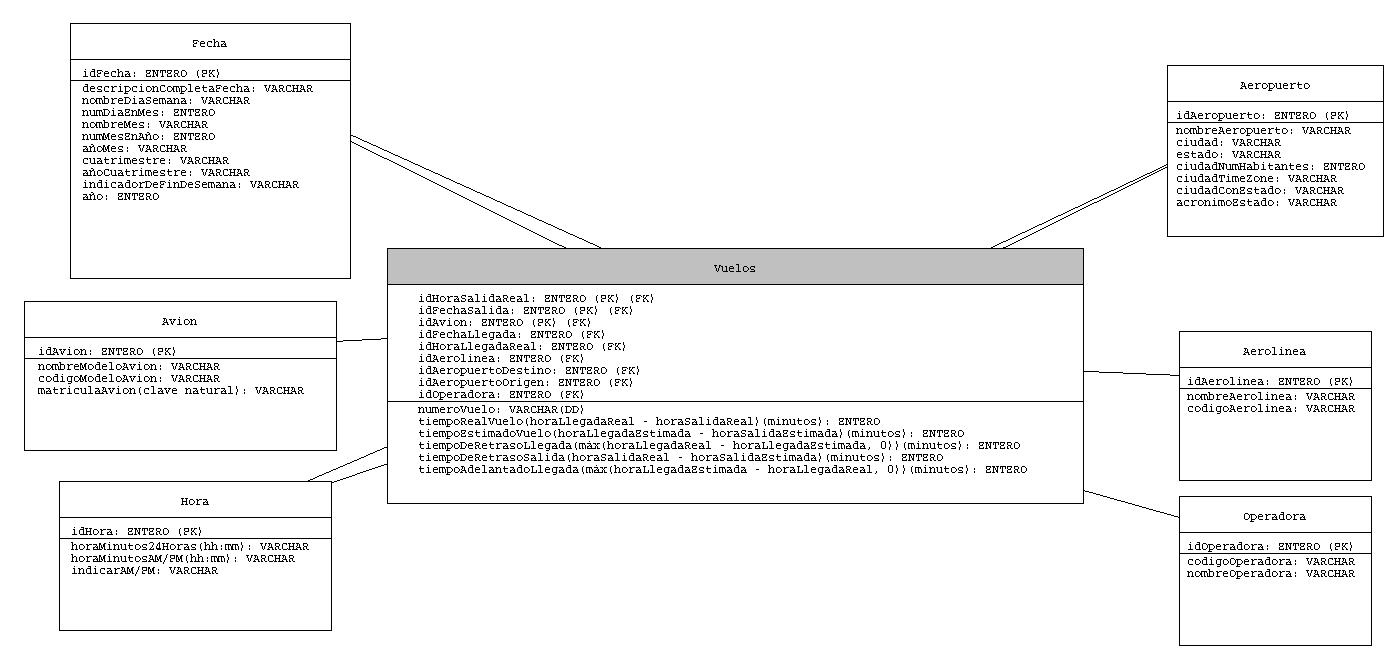
\includegraphics[scale=0.5]{images/esquema_estrella_modificado.jpg}
        \caption{Esquema en estrella modificado para albergar cambios de los aeropuertos}
        \label{fig:esquema_estrella_modificado}
    \end{figure}
    \newpage
    % Workflow vuelos
    \begin{figure}
        \centering
        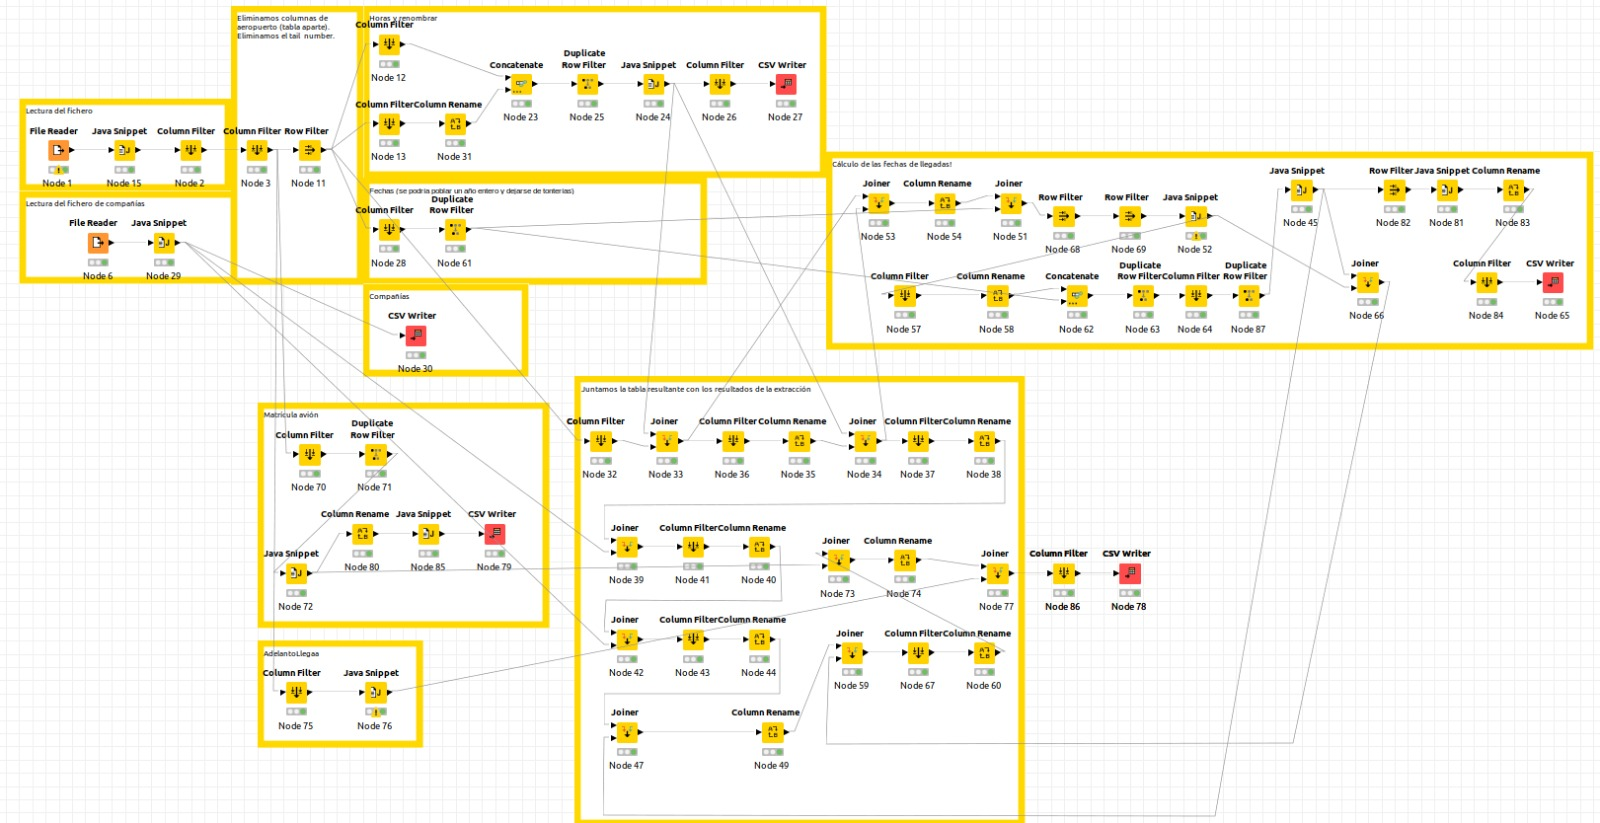
\includegraphics[scale=0.4]{images/workflow_vuelos.jpeg}
        \caption{\textit{Workflow} del fichero de vuelos}
        \label{fig:workflow_vuelos}
    \end{figure}
    \newpage
    \begin{figure}
        \centering
        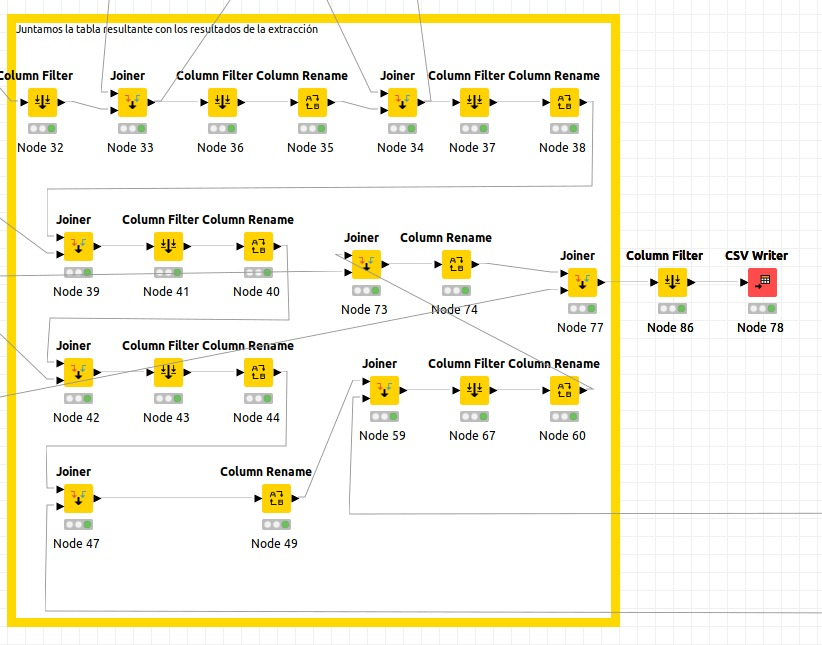
\includegraphics[scale=0.5]{images/workflow_vuelos_joins.jpeg}
        \caption{Parte del \textit{Workflow} de procesamiento del fichero de vuelos que se encarga de juntar los identificadores de las tablas de dimensión}
        \label{fig:workflow_vuelos_join}
    \end{figure}
    \newpage
    % Workflow ciudades y aeropuertos
    \begin{figure}
        \centering
        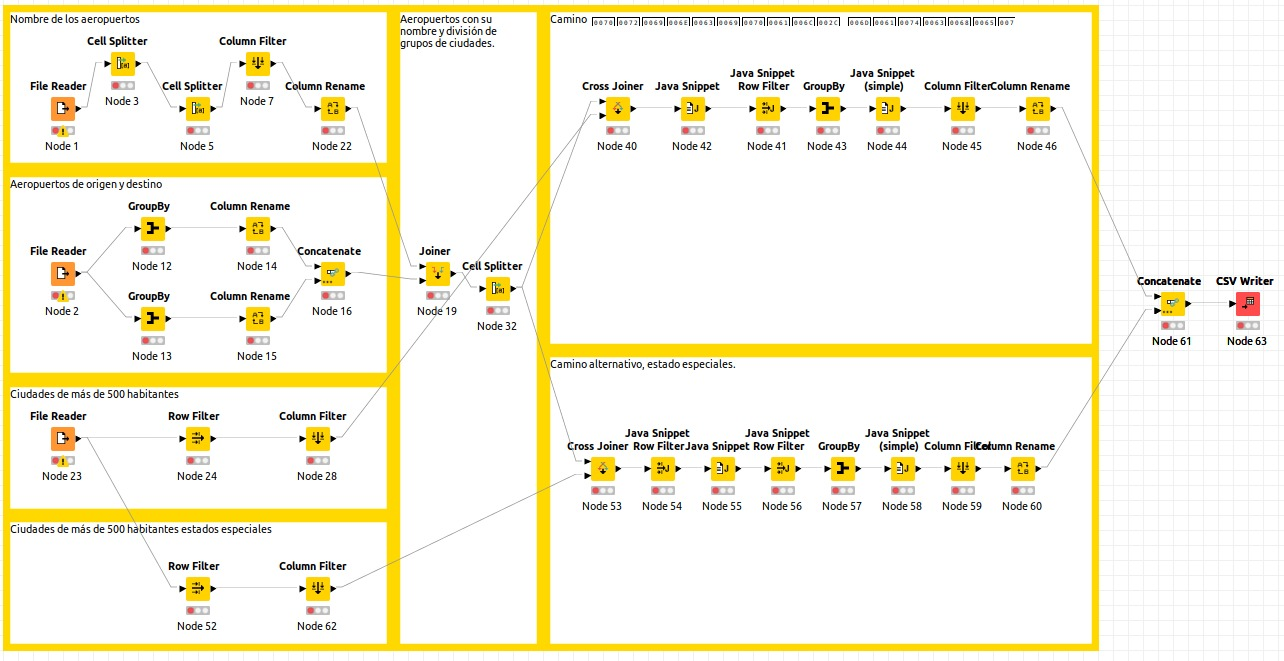
\includegraphics[scale=0.5]{images/workflow_ciudades.jpeg}
        \caption{\textit{Workflow} de procesamiento del fichero de aeropuertos y ciudades}
        \label{fig:workflow_aeropuertos_ciudades}
    \end{figure}
    \newpage
    \begin{figure}
        \centering
        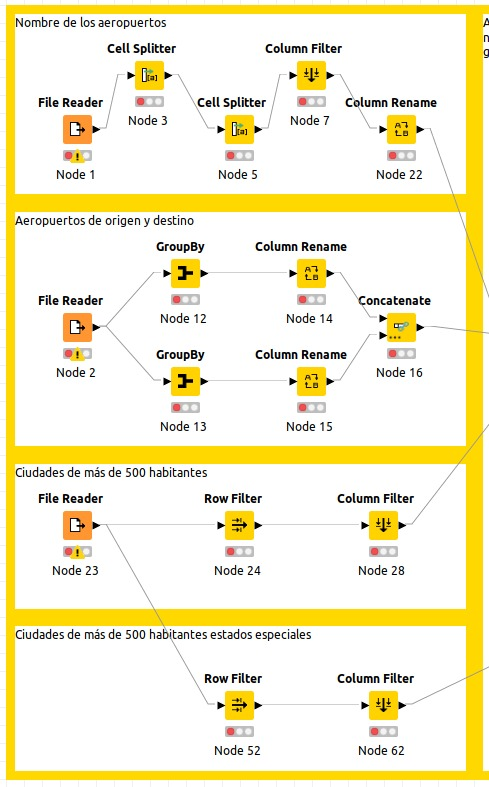
\includegraphics[scale=0.5]{images/workflow_ciudades_1.jpeg}
        \caption{Primera etapa del \textit{Workflow} de procesamiento de aeropuertos y ciudades}
        \label{fig:workflow_aeropuertos_ciudades_1}
    \end{figure}
    \newpage
    \begin{figure}
        \centering
        
\includegraphics[scale=0.5]{images/workflow_ciudades_2.jpeg}
        \caption{Segunda etapa del \textit{Workflow} de procesamiento de aeropuertos y ciudades}
        \label{fig:workflow_aeropuertos_ciudades_2}
    \end{figure}
    \newpage
    \begin{figure}
        \centering
        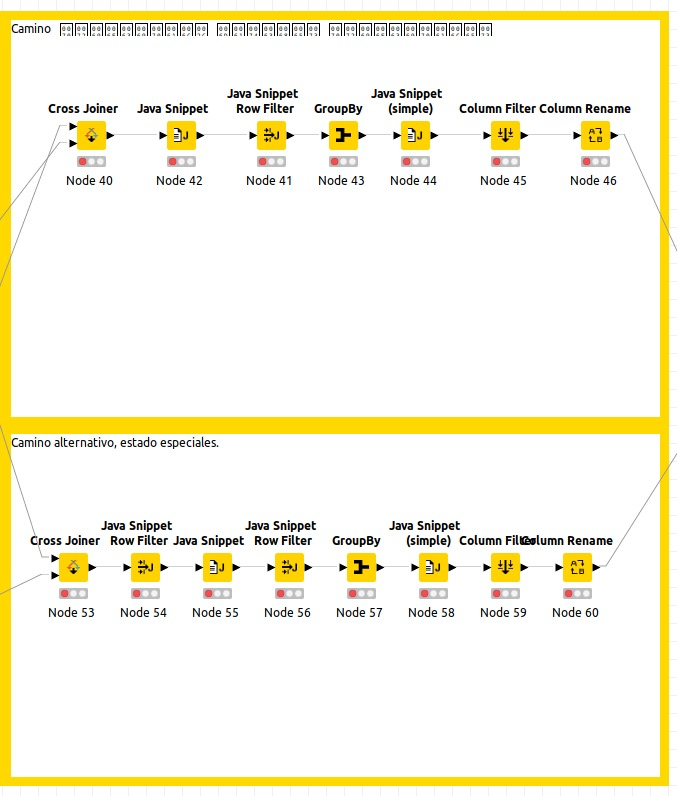
\includegraphics[scale=0.5]{images/workflow_ciudades_3.jpeg}
        \caption{Tercera etapa del \textit{Workflow} de procesamiento de aeropuertos y ciudades}
        \label{fig:workflow_aeropuertos_ciudades_3}
    \end{figure}
    \newpage
    \begin{figure}
        \centering
        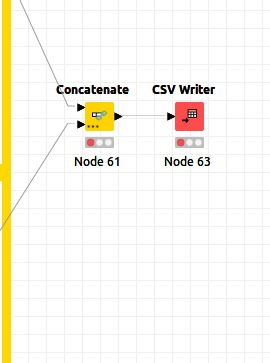
\includegraphics[scale=0.5]{images/workflow_ciudades_4.jpeg}
        \caption{Cuarta etapa del \textit{Workflow} de procesamiento de aeropuertos y ciudades}
        \label{fig:workflow_aeropuertos_ciudades_4}
    \end{figure}
\end{landscape}

% Anexo de codigos
\newpage
\section{Anexo 2: Códigos}

\lstinputlisting[label={list:codigoSQL}, caption={Código \textit{SQL} de creación de tablas}]{listings/createSQL.sql}

% Bibliografía
\newpage
\addcontentsline{toc}{section}{Referencias}
\bibliographystyle{unsrt}
\bibliography{bibliografia.bib}

\end{document}